\section{Creating a line of variations: \addbs{tkzTabVar}}
\subsection{Definition}

\begin{NewMacroBox}{tkzTabVar}{\oarg{local options}\var{el($1$),\dots,el($n$)}}
  with \tkzname{el($i$) = s($i$) / e($i$)} or \tkzname{el($i$) = s($i$) / eg($i$) / ed($i$)}.

\noindent\tkzname{s($i$)} is a sequence of symbols chosen from the table below. \tkzname{eg($i$)} and \tkzname{ed($i$)} are mathematical expressions placed on the left (\emph{gauche}) and on the right (\emph{droite}) of the vertical rules. \tkzname{e($i$)} is an expression centered on a rule.

\medskip
 \begin{tabular}{llrl}
\toprule
 Group 1& \emph{with one sign} &&\\
\midrule
\tkzname{s($i$)}  & Position of the expressions & \tkzname{el($i$)}  &      \\
\midrule
\IargName{tkzTabVar}{$-~~~$}& single expression, centered, at the bottom  eg=ed   &  $-   $&$/e    $    \\
\IargName{tkzTabVar}{$+~~~$}& single expression, centered, at the top eg=ed   &  $+   $&$/e    $    \\
\IargName{tkzTabVar}{$~R~~$}& nothing, go to the next expression           &  $~R  $&$(/)   $    \\
\IargName{tkzTabVar}{$-C$}  & continuous extension at the bottom, centered &  $-C  $&$/e    $    \\
\IargName{tkzTabVar}{$+C$}  & continuous extension at the top, centered&  $+C  $&$/e    $    \\
\IargName{tkzTabVar}{$-H$}  & expression at the bottom, centered, then forbidden zone  &  $-H  $&$/e    $    \\
\IargName{tkzTabVar}{$+H$}  & expression at the top, centered, then forbidden zone &  $+H  $&$/e    $    \\
\IargName{tkzTabVar}{$+D~~$}& discontinuity, expression at the top left        &  $+D  $&$/e    $    \\
\IargName{tkzTabVar}{$-D~~$}& discontinuity, expression at the bottom left         &  $-D  $&$/e    $    \\
\IargName{tkzTabVar}{$~D+~$}& discontinuity, expression at the top right     &  $D+  $&$/e    $    \\
\IargName{tkzTabVar}{$~D-~$}& discontinuity, expression at the bottom right        &  $D-  $&$/e    $    \\
\IargName{tkzTabVar}{$+DH$} & discontinuity on the left, at the top, then forbidden zone&  $+DH $&$/e    $  \\
\IargName{tkzTabVar}{$-DH$} & discontinuity on the left, at the bottom, then forbidden zone &  $-DH $&$/e    $    \\
\IargName{tkzTabVar}{$+CH$} & continuous extension then forbidden zone    &  $+CH $&$/e    $    \\
\IargName{tkzTabVar}{$-CH$} & same, but expression at the bottom left           &  $-CH $&$/e    $    \\
\midrule
 Group 2& \emph{with two signs}& &\\
\midrule
\IargName{tkzTabVar}{$+D-$} & discontinuity,\hfill two expressions    &  $+D- $&$/eg/ed$    \\
\IargName{tkzTabVar}{$-D+$} & discontinuity, \dots \hfill      that are    &  $-D+ $&$/eg/ed$    \\
\IargName{tkzTabVar}{$+D+$} & discontinuity, \dots \hfill either on the left or on the right &$+D+ $&$/eg/ed$    \\
\IargName{tkzTabVar}{$-D-$} & discontinuity, \dots \hfill either at the top or at the bottom&$-D- $&$/eg/ed$    \\
\IargName{tkzTabVar}{$+CD+$}& continuous extension on the left and          &  $+CD+$&$/eg/ed$    \\
\IargName{tkzTabVar}{$-CD-$}& \dots \hfill  two expressions that are        &  $-CD-$&$/eg/ed$    \\
\IargName{tkzTabVar}{$+CD-$}& \dots \hfill  either on the left or on the right  &  $+CD-$&$/eg/ed$    \\
\IargName{tkzTabVar}{$-CD+$}& \dots \hfill   either at the top or at the bottom   &  $-CD+$&$/eg/ed$    \\
\IargName{tkzTabVar}{$+DC+$}& continuous extension on the right and           &  $+DC+$&$/eg/ed$    \\
\IargName{tkzTabVar}{$-DC-$}& \dots \hfill  two expressions that are          &  $-DC-$&$/eg/ed$    \\
\IargName{tkzTabVar}{$+DC-$}& \dots \hfill  either on the left or on the right      &  $+DC-$&$/eg/ed$    \\
\IargName{tkzTabVar}{$-DC+$}& \dots \hfill   either at the top or at the bottom         &  $-DC+$&$/eg/ed$    \\
\IargName{tkzTabVar}{$+V+$} & like a discontinuity but without double bar, and&  $+V+ $&$/eg/ed$    \\
\IargName{tkzTabVar}{$-V-$} & \dots \hfill  two expressions that are     &  $-V- $&$/eg/ed$    \\
\IargName{tkzTabVar}{$+V-$} & \dots \hfill  either on the left or on the right &  $+V- $&$/eg/ed$    \\
\IargName{tkzTabVar}{$-V+$} & \dots \hfill   either at the top or at the bottom    &  $-V+ $&$/eg/ed$    \\
\midrule
\tkzname{\textvisiblespace} & leaves the place empty in some cases& &   \\
\bottomrule
\end{tabular}

\medskip
\noindent\emph{The macro \tkzcname{tkzTabVar} takes one argument: a list. This list has \tkzname{$n$} elements, matching the \tkzname{$n$} values of the first row. Each element gives the position of one or two expressions in the row: a sign $+$ (at the top) or a sign $-$ (at the bottom). These expressions are values of the function or limits.}

\noindent\emph{The elements \tkzname{el($i$)} have the form:\\
 either \mbox{\tkzname{\{ s($i$)/ e($i$)\}}} or \mbox{\tkzname{\{ s($i$)/ e($i$) / \}}}, or \mbox{\tkzname{\{ s($i$)/ eg($i$) / ed($i$)\}}}.}

\noindent\emph{The first form is for the symbols that have only one sign \tkzname{$+$} or \tkzname{$-$} and place a single expression; the second is for the symbols that have two signs and place two expressions. The expressions are values taken by the function on the left \tkzname{eg($i$)} or on the right \tkzname{ed($i$)}, or limits; they can also be empty. A sign \tkzname{$+$} or \tkzname{$-$} on the left (resp. on the right) of the symbol corresponds to \tkzname{eg($i$)} (resp. \tkzname{ed($i$)}).}

\medskip
\begin{tabular}{lllc}
\toprule
\texttt{options}               & \texttt{default} & \texttt{definition}              \\
\midrule
\IoptName{tkzTabVar}{color}  & |black|         & color of the arrows                \\
\IoptName{tkzTabVar}{help}   & |false| & shows the structure of a line of variations      \\
 \bottomrule
\end{tabular}

\end{NewMacroBox}

 \medskip
A picture is sometimes better than a long speech\dots

 \begin{center}
\begin{tikzpicture}
\tkzTabInit[lgt=2,espcl=3]{$x$/1,$f'(x)$/1,$f(x)$/3}%
{$0$,$1$,$2$,$+\infty$}%
\tkzTabLine{t,-,d,-,z,+,}%
\tkzTabVar{}%
\node[below =3pt]  (FN12) at (N12){};
\node[below =3pt]  (FN22) at (N22){};
\node[below =3pt]  (FN32) at (N32){};
\node[below =3pt]  (FN42) at (N42){};

\node[above =3pt]  (FN13) at (N13){};
\node[above =3pt]  (FN23) at (N23){};
\node[above =3pt]  (FN33) at (N33){};
\node[above =3pt]  (FN43) at (N43){};

\node[below right=3pt]  (FRN12) at (N12){};
\node[below right=3pt]  (FRN22) at (N22){};
\node[below right=3pt]  (FRN32) at (N32){};
\node[below right=3pt]  (FRN42) at (N42){};

\node[above right=3pt]  (FRN13) at (N13){};
\node[above right=3pt]  (FRN23) at (N23){};
\node[above right=3pt]  (FRN33) at (N33){};

\node[below left=3pt]  (FLN22) at (N22){};
\node[below left=3pt]  (FLN32) at (N32){};
\node[below left=3pt]  (FLN42) at (N42){};

\node[above left=3pt]  (FLN13) at (N13){};
\node[above left=3pt]  (FLN23) at (N23){};
\node[above left=3pt]  (FLN33) at (N33){};
\node[above left=3pt]  (FLN43) at (N43){};

\draw[fill=red!50] (FN12) circle(2pt)  node[below=2pt,text=red!50] {\small e} node[left=1cm,red] {$+$};
\draw[fill=red!50] (FN22) circle(2pt);
\draw[fill=red!50] (FN32) circle(2pt);
\draw[fill=red!50] (FN42) circle(2pt);

\draw[fill=red!50] (FN13) circle(2pt)  node[left=1cm,red] {$-$};
\draw[fill=red!50] (FN23) circle(2pt);
\draw[fill=red!50] (FN33) circle(2pt) node[above=2pt,text=red!50] {\small e};
\draw[fill=red!50] (FN43) circle(2pt);

\draw[fill=blue!30] (FRN12) circle(2pt);
\draw[fill=blue!30] (FRN22) circle(2pt) node[below right=2pt,text=blue!30] {\small ed};
\draw[fill=blue!30] (FRN32) circle(2pt);
\draw[fill=blue!30] (FRN13) circle(2pt);
\draw[fill=blue!30] (FRN23) circle(2pt);
\draw[fill=blue!30] (FRN33) circle(2pt);

\draw[fill=green!50] (FLN22) circle(2pt);
\draw[fill=green!50] (FLN32) circle(2pt);
\draw[fill=green!50] (FLN42) circle(2pt) node[below left =2pt,text=green!50] {\small eg};
\draw[fill=green!50] (FLN23) circle(2pt) node[above left =2pt,text=green!50] {\small eg};
\draw[fill=green!50] (FLN33) circle(2pt);
\draw[fill=green!50] (FLN43) circle(2pt);
\end{tikzpicture}
\end{center}

\medskip
For some of the tables, I used the following macros:

\begin{tkzexample}[code only]
	\newcommand*{\va}{\colorbox{red!50}    {$\scriptscriptstyle V_a$}}
	\newcommand*{\vb}{\colorbox{blue!50}   {$\scriptscriptstyle V_b$}}
	\newcommand*{\vbo}{\colorbox{blue!50}  {$\scriptscriptstyle V_{b1}$}}
	\newcommand*{\vbt}{\colorbox{yellow!50}{$\scriptscriptstyle V_{b2}$}}
	\newcommand*{\vc}{\colorbox{gray!50}   {$\scriptscriptstyle V_c$}}
	\newcommand*{\vd}{\colorbox{magenta!50}{$\scriptscriptstyle V_d$}}
	\newcommand*{\ve}{\colorbox{orange!50} {$\scriptscriptstyle V_e$}}
\end{tkzexample}

\medskip
 \begin{center}
\begin{tikzpicture}
\tkzTabInit[lgt=2,espcl=3]{$x$/1,$f'(x)$/1,$f(x)$/3}%
{$0$,$1$,$2$,$+\infty$}%
  \tkzTabLine{t,-,d,-,z,+,}%
	\tkzTabVar{+/\va , -D+/\vb/\vc,-/\vd, +D/\ve}%
\end{tikzpicture}
\end{center}

\begin{tkzexample}[code only]
	\begin{tikzpicture}
	\tkzTabInit[lgt=2,espcl=3]{$x$/1,$f'(x)$/1,$f(x)$/3}%
	{$0$,$1$,$2$,$+\infty$}%
\tkzTabLine{t,-,d,-,z,+,}%
	\tkzTabVar{+/\va , -D+/\vb/\vc,-/\vd, +D/\ve}%
\end{tikzpicture}
\end{tkzexample}

Comments: the signs $+$ and $-$ place an end of the arrow at the top or at the bottom of the row. With a single sign, a single expression is needed. Its position with respect to the column is given by the position of the sign with respect to the other symbols (see \tkzname{$+D$}). \tkzname{$-D+$} needs two expressions.

\subsection{Using the symbols}

\medskip
\bgroup\parindent=0pt
\begin{minipage}{7cm}
\begin{tkzexample}[code only]
 {+ /\va , -/\vb }
\end{tkzexample}
  \begin{tikzpicture}
  \tkzTabInit[lgt=1]{ /0.5,/2 }{ a , b }
  \tkzTabVar%
  {+ /\va , -/\vb }
  \end{tikzpicture}
\end{minipage}
\hfill
\begin{minipage}{7cm}
\begin{tkzexample}[code only]
 {-/\va   ,   +/\vb}
\end{tkzexample}
  \begin{tikzpicture}
  \tkzTabInit[lgt=1]{ /0.5,/2 }{ a , b }
  \tkzTabVar%
{-/\va   ,   +/\vb}
  \end{tikzpicture}
\end{minipage}

\begin{minipage}{7cm}
\begin{tkzexample}[code only]
 {+/\va   ,   +/\vb}
\end{tkzexample}
  \begin{tikzpicture}
  \tkzTabInit[lgt=1]{ /0.5,/2 }{ a , b }
  \tkzTabVar%
{+/\va   ,   +/\vb}
  \end{tikzpicture}
\end{minipage}
\hfill
\begin{minipage}{7cm}
\begin{tkzexample}[code only]
 {-/\va   ,   -/\vb}
\end{tkzexample}
  \begin{tikzpicture}
  \tkzTabInit[lgt=1]{ /0.5,/2 }{ a , b }
  \tkzTabVar%
{-/\va   ,   -/\vb}
  \end{tikzpicture}
\end{minipage}

\begin{minipage}{7cm}
\begin{tkzexample}[code only]
 {+/\va  , -C / \vb}
\end{tkzexample}
  \begin{tikzpicture}
  \tkzTabInit[lgt=1]{ /0.5,/2 }{ a , b }
  \tkzTabVar%
{+/\va  , -C / \vb}
  \end{tikzpicture}
\end{minipage}
\hfill
\begin{minipage}{7cm}
\begin{tkzexample}[code only]
{-/\va  , +C / \vb }\end{tkzexample}
  \begin{tikzpicture}
  \tkzTabInit[lgt=1]{ /0.5,/2 }{ a , b }
  \tkzTabVar%
{-/\va  , +C / \vb }
  \end{tikzpicture}
\end{minipage}

\begin{minipage}{7cm}
\begin{tkzexample}[code only]
 {+C  / \va ,  -C / \vb}
\end{tkzexample}
\begin{tikzpicture}
  \tkzTabInit[lgt=1]{ /0.5,/2 }{ a , b }
   \tkzTabVar%
 {+C  / \va ,  -C / \vb }
\end{tikzpicture}
\end{minipage}
\hfill
\begin{minipage}{7cm}
\begin{tkzexample}[code only]
 {-C /\va  , +C /\vb}
\end{tkzexample}
\begin{tikzpicture}
  \tkzTabInit[lgt=1]{ /0.5,/2 }{ a , b }
     \tkzTabVar%
 {-C /\va  , +C /\vb}
\end{tikzpicture}
\end{minipage}

\begin{minipage}{7cm}
\begin{tkzexample}[code only]
 { D+  /\va  ,  -/\vb}
\end{tkzexample}
  \begin{tikzpicture}
  \tkzTabInit[lgt=1]{ /0.5,/2 }{ a , b }
  \tkzTabVar%
 { D+  /\va  ,  -/\vb}
  \end{tikzpicture}
\end{minipage}
\hfill
\begin{minipage}{7cm}
\begin{tkzexample}[code only]
 { D-  /\va  ,  +/\vb}
\end{tkzexample}
  \begin{tikzpicture}
  \tkzTabInit[lgt=1]{ /0.5,/2 }{ a , b }
  \tkzTabVar
  { D-  /\va  ,  +/\vb}
  \end{tikzpicture}
\end{minipage}

\begin{minipage}{7cm}
\begin{tkzexample}[code only]
 {+/\va  , -D / \vb}
\end{tkzexample}
  \begin{tikzpicture}
  \tkzTabInit[lgt=1]{ /0.5,/2 }{ a , b }
  \tkzTabVar%
{+/\va  , -D / \vb}
  \end{tikzpicture}
\end{minipage}
\hfill
\begin{minipage}{7cm}
\begin{tkzexample}[code only]
 {-/\va  , +D / \vb }
\end{tkzexample}
  \begin{tikzpicture}
  \tkzTabInit[lgt=1]{ /0.5,/2 }{ a , b }
  \tkzTabVar%
{-/\va  , +D / \vb }
  \end{tikzpicture}
\end{minipage}

\begin{minipage}{7cm}
\begin{tkzexample}[code only]
 {D+ / \va , -D / \vb }
\end{tkzexample}
\begin{tikzpicture}
  \tkzTabInit[lgt=1]{ /0.5,/2 }{ a , b }
   \tkzTabVar%
 {D+  / \va ,  -D / \vb }
\end{tikzpicture}
\end{minipage}
\hfill
\begin{minipage}{7cm}
\begin{tkzexample}[code only]
 {D- /\va , +D /\vb}
\end{tkzexample}
\begin{tikzpicture}
  \tkzTabInit[lgt=1]{ /0.5,/2 }{ a , b }
     \tkzTabVar%
 {D- /\va  , +D /\vb}
\end{tikzpicture}
\end{minipage}

\begin{minipage}{7cm}
\begin{tkzexample}[code only]
 {+/ \va , -/ \vb , +/ \vc}
\end{tkzexample}
\begin{tikzpicture}
\tkzTabInit[lgt=1,espcl=2.5]{ /0.5,/2 }{ a , b , c }
\tkzTabVar  {+/ \va , -/  \vb ,+/  \vc}
\end{tikzpicture}
\end{minipage}
\hfill
\begin{minipage}{7cm}
\begin{tkzexample}[code only]
 {+/ \va ,-C/ \vb , +/  \vc/ }
\end{tkzexample}
\begin{tikzpicture}
\tkzTabInit[lgt=1,espcl=2.5]{ /0.5,/2 }{ a , b , c }
\tkzTabVar {+/ \va  ,-C/ \vb , +/  \vc/ }
\end{tikzpicture}
\end{minipage}

\begin{minipage}{7cm}
\begin{tkzexample}[code only]
 {-  /\va , R , +/\vc}
\end{tkzexample}
\begin{tikzpicture}
\tkzTabInit[lgt=1,espcl=2.5]{ /0.5,/2 }{ a , b , c }
\tkzTabVar%
{-  /\va  ,  R,  +/\vc}
\end{tikzpicture}
\end{minipage}
\hfill
\begin{minipage}{7cm}
\begin{tkzexample}[code only]
 {-  /\va , R , +/\vc}
\end{tkzexample}
\begin{tikzpicture}
\tkzTabInit[lgt=1,espcl=2.5]{ /0.5,/2}{ a , b , c }
\tkzTabVar%
{-  /\va  ,  R  ,  +/\vc}
\end{tikzpicture}
\end{minipage}

\begin{minipage}{7cm}
\begin{tkzexample}[code only]
 {D-/\va , +DH/\vbo/ , }
\end{tkzexample}
\begin{tikzpicture}
\tkzTabInit[lgt=1,espcl=2.5]{ /0.5,/2 }{ a , b , c }
\tkzTabVar%
{D-/\va  ,  +DH/\vbo/ ,  }
\end{tikzpicture}
\end{minipage}
\hfill
\begin{minipage}{7cm}
\begin{tkzexample}[code only]
 {D-/\va  , -DH/\va/\vb ,  D+/}
\end{tkzexample}
\begin{tikzpicture}
\tkzTabInit[lgt=1,espcl=2.5]{ /0.5,/2 }{ a , b , c }
\tkzTabVar%
{D-/\va  ,  -DH/\vbo ,  D+/}
\end{tikzpicture}
\end{minipage}

\begin{minipage}{7cm}
\begin{tkzexample}[code only]
 {D-/\va , +D-/\vbo/\vbt , +D/\vc}
\end{tkzexample}
\begin{tikzpicture}
\tkzTabInit[lgt=1,espcl=2.5]{ /0.5,/2 }{ a , b , c }
\tkzTabVar%
{D-/\va  ,  +D-/\vbo/\vbt , +D/\vc}
\end{tikzpicture}
\end{minipage}
\hfill
\begin{minipage}{7cm}
\begin{tkzexample}[code only]
 {D-/\va , +D-/\vbo/\vbt , +D/\vc}
\end{tkzexample}
\begin{tikzpicture}
\tkzTabInit[lgt=1,espcl=2.5]{ /0.5,/2 }{ a , b , c }
\tkzTabVar%
{D-/\va  ,  -D-/\vbo/\vbt , +D/\vc}
\end{tikzpicture}
\end{minipage}

\begin{minipage}{7cm}
\begin{tkzexample}[code only]
 {+/\va , -D- / \vbo/\vbt , +/\vc}
\end{tkzexample}
\begin{tikzpicture}
\tkzTabInit[lgt=1,espcl=2.5]{ /0.5,/2 }{ a , b , c }
\tkzTabVar  {+/ \va , -D- /\vbo/\vbt,+/\vc  }
\end{tikzpicture}
\end{minipage}
\hfill
\begin{minipage}{7cm}
\begin{tkzexample}[code only]
 {+ /\va,-DC- /\vbo/\vbt,+ /\vc}
\end{tkzexample}
\begin{tikzpicture}\tikzset{low/.style   = {above  =  15pt}}
\tkzTabInit[lgt=1,espcl=2.5]{ /0.5,/2 }{ a , b , c }
\tkzTabVar {+   /\va ,-DC- /\vbo/\vbt  ,+ /\vc}
\end{tikzpicture}
\end{minipage}

\begin{minipage}{7cm}
\begin{tkzexample}[code only]
 {D-/\va, +DC-/\vbo/\vbt, +D/\vc}
\end{tkzexample}
\begin{tikzpicture}
\tkzTabInit[lgt=1,espcl=2.5]{ /0.5,/2 }{ a , b , c }
\tkzTabVar%
{D-/\va  ,  +DC-/\vbo/\vbt ,+D/\vc}
\end{tikzpicture}
\end{minipage}
\hfill
\begin{minipage}{7cm}
\begin{tkzexample}[code only]
 {D+/\va , +DC-/\vbo/\vbt , +D/\vc}
\end{tkzexample}
\begin{tikzpicture}
\tkzTabInit[lgt=1,espcl=2.5]{ /0.5,/2 }{ a , b , c }
\tkzTabVar%
{D+/\va  ,  +DC-/\vbo/\vbt ,+D/\vc}
\end{tikzpicture}
\end{minipage}

\begin{minipage}{7cm}
\begin{tkzexample}[code only]
 {D-/\va , +CD-/\vbo/\vbt , +D/\vc}
\end{tkzexample}
\begin{tikzpicture}
\tkzTabInit[lgt=1,espcl=2.5]{ /0.5,/2 }{ a , b , c }
\tkzTabVar%
{D-/\va  ,  +CD-/\vbo/\vbt , +D/\vc}
\end{tikzpicture}
\end{minipage}
\hfill
\begin{minipage}{7cm}
\begin{tkzexample}[code only]
 {D-/\va , +CD-/\vbo/\vbt ,+D/\vc}
\end{tkzexample}
\begin{tikzpicture}
\tkzTabInit[lgt=1,espcl=2.5]{ /0.5,/2 }{ a , b , c }
\tkzTabVar%
{D+/\va , +CD-/\vbo/\vbt ,  +D/\vc}
\end{tikzpicture}
\end{minipage}

\begin{minipage}{7cm}
\begin{tkzexample}[code only]
 {+/\va, -DC+ /\vbo/\vbt, - /\vc}
\end{tkzexample}
\begin{tikzpicture}
\tkzTabInit[lgt=1,espcl=2.5]{ /0.5,/2 }{ a , b , c }
\tkzTabVar  {+ /\va ,-DC+ /\vbo/\vbt , -/\vc}
\end{tikzpicture}
\end{minipage}
\hfill
\begin{minipage}{7cm}
\begin{tkzexample}[code only]
 {D- /\va, -DC- /\vbo/\vbt,+D/\vc}
\end{tkzexample}
\begin{tikzpicture}\tikzset{low/.style           = {above       =  15pt}}
\tkzTabInit[lgt=1,espcl=2.5]{ /0.5,/2 }{ a , b , c }
\tkzTabVar%
{D- /\va  , -DC- /\vbo/\vbt , +D/\vc}
\end{tikzpicture}
\end{minipage}

\begin{minipage}{7cm}
\begin{tkzexample}[code only]
 {+/\va  , -CH /\vbo/\vbt , D+/}
\end{tkzexample}
\begin{tikzpicture}
\tkzTabInit[lgt=1,espcl=2.5]{ /0.5,/2 }{ a , b , c }
\tkzTabVar%
{+/\va  , -CH /\vbo/\vbt , D+/}
\end{tikzpicture}
\end{minipage}
\hfill
\begin{minipage}{7cm}
\begin{tkzexample}[code only]
 {+  /\va  , -CH/\vb,  //}
\end{tkzexample}
\begin{tikzpicture}
\tkzTabInit[lgt=1,espcl=2.5]{ /0.5,/2 }{ a , b , c }
\tkzTabVar%
{+  /\va  , -CH/\vb,  //}
\end{tikzpicture}
\end{minipage}

\begin{minipage}{7cm}
\begin{tkzexample}[code only]
 {+/\va , -V- /\vbo /\vbt, +/\vc}
\end{tkzexample}
\begin{tikzpicture}
\tkzTabInit[lgt=1,espcl=2.5]{ /0.5,/2 }{ a , b , c }
\tkzTabVar  {+/\va,-V- /\vbo /\vbt, +/\vc}
\end{tikzpicture}
\end{minipage}
\hfill
\begin{minipage}{7cm}
\begin{tkzexample}[code only]
 {+/ \va ,-V+ / \vbo/ \vbt ,-/ \vc}
\end{tkzexample}
\begin{tikzpicture}
\tkzTabInit[lgt=1,espcl=2.5]{ /0.5,/2 }{ a , b , c }
\tkzTabVar  {+/ \va ,-V+ / \vbo/ \vbt ,-/ \vc}
\end{tikzpicture}
\end{minipage}

\begin{minipage}{7cm}
\begin{tkzexample}[code only]
 {+/ \va ,+V- /\vbo/ \vbt , -/\vc}
\end{tkzexample}
\begin{tikzpicture}
\tkzTabInit[lgt=1,espcl=2.5]{ /0.5,/2 }{ a , b , c }
\tkzTabVar  {+/ \va ,+V- / \vbo/ \vbt , -/\vc}
\end{tikzpicture}
\end{minipage}
\hfill
\begin{minipage}{7cm}
\begin{tkzexample}[code only]
 {-/ \va, +V+ / \vbo/\vbt, -/\vc}
\end{tkzexample}
\begin{tikzpicture}
\tkzTabInit[lgt=1,espcl=2.5]{ /0.5,/2 }{ a , b , c }
\tkzTabVar  {-/ \va ,+V+ / \vbo / \vbt, -/\vc}
\end{tikzpicture}
\end{minipage}

\begin{minipage}{16cm}
\begin{tkzexample}[code only]
 {-/ \va ,+H/\vb,-/\vc, +/ \vd}
\end{tkzexample}
\begin{tikzpicture}
\tkzTabInit[lgt=1,espcl=3]{ /0.5,/2 }{ a , b , c , d }
\tkzTabVar  {-/  \va  ,+H/\vb,-/\vc, +/  \vd}
\end{tikzpicture}
\end{minipage}

\begin{minipage}{16cm}
\begin{tkzexample}[code only]
 {+/  \va  ,-H/\vb,-/\vc, +/  \vd}
\end{tkzexample}
\begin{tikzpicture}
\tkzTabInit[lgt=1,espcl=3]{ /0.5,/2 }{ a , b , c , d }
\tkzTabVar  {+/  \va  ,-H/\vb,-/\vc, +/  \vd}
\end{tikzpicture}
\end{minipage}

\begin{minipage}{16cm}
\begin{tkzexample}[code only]
 {-/  \va  , R , R , R , +/  \ve}
\end{tkzexample}
\begin{tikzpicture}
\tkzTabInit[lgt=1,espcl=3]{ /0.5,/2 }{ a , b , c , d , e}
\tkzTabVar  {-/  \va  ,R,R,R, +/  \ve}
\end{tikzpicture}
\end{minipage}

\begin{minipage}{16cm}
\begin{tkzexample}[code only]
  {-/ \va , +/\vb , -DH/\vc , -/\vd , +/ \ve}
 \end{tkzexample}
\begin{tikzpicture}
\tkzTabInit[lgt=1,espcl=3]{ /0.5,/2 }{ a , b , c , d , e}
\tkzTabVar  {-/ \va  ,+/\vb ,-DH/\vc,-/\vd, +/ \ve}
\end{tikzpicture}
\end{minipage}

\begin{minipage}{16cm}
\begin{tkzexample}[code only]
 {D-/ \va , +DH/\vb/ , D-/\vc , +/\vd , +D/\ve}
\end{tkzexample}
\begin{tikzpicture}
\tkzTabInit[lgt=1,espcl=3]{ /0.5,/2 }{ a , b , c , d , e}
\tkzTabVar  {D-/  \va ,+DH/\vb/,D-/\vc,+/\vd, -D/\ve}
\end{tikzpicture}
\end{minipage}
\egroup

\medskip
Comments
\begin{itemize}
  \item the syntax $s(i)/\ldots/\ldots$ can be used in almost every case, but then the expressions must be placed correctly;

  \item the empty argument is sometimes used at the end of a row, but then no arrow is drawn;

  \item $C+$ and $C-$ do not exist: $+C$ and $-C$ are enough because the expressions are centered;
  \item $D+$ and $D-$ do exist.

\end{itemize}


\subsection{Using the options}

\subsubsection{\texttt{\textcolor{red}{color}}: color of the arrows}
The table can be customized with styles.
\begin{tkzexample}[vbox, small]
\begin{tikzpicture}
  \tkzTabInit[color,espcl=8]%
    {$x$   /1,%
     Sign\\ of $\dfrac{1}{x}$ /1.5,
     Variations\\ of $\ln$      /1.5}%
    {$0$,$+\infty$}%
  \tkzTabLine{d,+,}%
  \tkzTabVar[color=red]%
    {D-/    /  $-\infty$,+/  $+\infty$  /}
\end{tikzpicture}
\end{tkzexample}

\subsubsection{\texttt{\textcolor{red}{help}}: shows the structure of the table}
\Iopt{tkzTabVar}{help}
See the section ``Customizing the tables'' (\ref{pers}).
\subsection{Using the styles}

\subsubsection{Color of a forbidden zone}
\Istyle{tkzTabvar}{h style}
To color or hatch a zone of the table in another way, change a style.

By default, \tkzname{h style} is defined as follows:
\begin{tkzexample}[code only]
 \tikzset{h style/.style = {fill=gray,opacity=0.4}}
\end{tkzexample}

Another definition could be:

\begin{tkzexample}[code only]
 \tikzset{h style/.style = {fill=red!50}}
\end{tkzexample}

\begin{tkzexample}[vbox,width=9cm]
\begin{tikzpicture}
 \tikzset{h style/.style = {fill=red!50}}
 \tkzTabInit[lgt=1,espcl=2]{$x$ /1,  $f$ /2}{$0$,$1$,$2$,$3$}%
 \tkzTabVar{+/ $1$  / , -CH/ $-2$ / , +C/  $5$, -/ $0$  /  }
\end{tikzpicture}
\end{tkzexample}

\subsubsection{\texttt{\textcolor{red}{h style}}: hatched forbidden zone}
\Istyle{tkzTabVar}{h style}

\begin{tkzexample}[code only]
  \tikzset{h style/.style = {pattern=north west lines}}
\end{tkzexample}
 This code hatches the zone.

\begin{tkzexample}[vbox,width=9cm,small]
\begin{tikzpicture}
 \tikzset{h style/.style = {pattern=north west lines}}
 \tkzTabInit[lgt=1,espcl=2]{$x$ /1,  $f$ /2}{$0$,$1$,$2$,$3$}%
 \tkzTabVar{+/ $1$  / , -CH/ $-2$ / , +C/  $5$, -/ $0$  /  }
\end{tikzpicture}
\end{tkzexample}


\subsubsection{\texttt{\textcolor{red}{arrow style}}: style of the arrows}
\Istyle{tkzTabVar}{arrow}
The style of the arrows is \tkzname{arrow style}; it is defined as follows:

\begin{tkzexample}[code only]
   \tikzset{arrow style/.style   = {\cmdTAB@VA@color,
                                    ->,
                                    >           = latex',
                                    shorten >   =  2pt,
                                    shorten <   =  2pt}}
\end{tkzexample}

 The arrows stop short of the nodes. Here is a possible change of the style:

\begin{tkzexample}[code only]
  \tikzset{arrow style/.style   = {blue,
                                   ->,
                                   >           = latex',
                                   shorten >   =  6pt,
                                   shorten <   =  6pt}}
\end{tkzexample}

 The color of the arrows and the gap at their ends are changed.

\begin{tkzexample}[vbox,small]
\begin{tikzpicture}
  \tikzset{arrow style/.style   = {blue,
                                   ->,
                                   >           = latex',
                                   shorten >   =  6pt,
                                   shorten <   =  6pt}}
  \tkzTabInit[espcl=5]{$x$ /1, $\ln x +1$ /1.5, $x \ln x$ /2}%
     {$0$ ,$1/\E$ , $+\infty$}%
  \tkzTabLine{d,-,z,+,}
  \tkzTabVar%
  { D+/   / $0$ ,%
     -/ \colorbox{black}{\textcolor{white}{$\dfrac{-1}{e}$}}/ ,%
     +/ $+\infty$  /  }%
\end{tikzpicture}
\end{tkzexample}

\subsubsection{\texttt{\textcolor{red}{node style}}: style of the nodes}
\Istyle{tkzTabVar}{node style}
The style of the nodes is \tkzname{node style}; by default it is defined as follows:
\begin{tkzexample}[code only]
\tikzset{node style/.style    = {inner sep   =  2pt,
                                 outer sep   =  2pt,
                                 fill        =  \cmdTAB@tbs@colorT}}\end{tkzexample}
To change it while keeping part of this style, you can write:

\begin{tkzexample}[code only]
  \tikzset{node style/.append style = {draw,circle,fill=red!40,opacity=.4}}
\end{tkzexample}

 By default, the nodes are rectangles that are not drawn; here they become disks.

\begin{tikzpicture}
  	\tikzset{node style/.append style    = {draw,circle,fill=red!40,opacity=.4}}
  \tkzTabInit[espcl=5]{$x$ /1, $\ln x +1$ /1.5, $x \ln x$ /2}%
     {$0$ ,$1/\E$ , $+\infty$}%
  \tkzTabLine{d,-,z,+,}
  \tkzTabVar%
  { D+/   / $0$ ,%
     -/ \colorbox{black}{\textcolor{white}{$\dfrac{-1}{e}$}}/ ,%
     +/ $+\infty$  /  }%
\end{tikzpicture}

\begin{tkzexample}[code only,small]
\begin{tikzpicture}
  	\tikzset{node style/.append style    = {draw,circle,fill=red!40,opacity=.4}}
  \tkzTabInit[espcl=5]{$x$ /1, $\ln x +1$ /1.5, $x \ln x$ /2}%
     {$0$ ,$1/\E$ , $+\infty$}%
  \tkzTabLine{d,-,z,+,}
  \tkzTabVar%
  { D+/   / $0$ ,%
     -/ \colorbox{black}{\textcolor{white}{$\dfrac{-1}{e}$}}/ ,%
     +/ $+\infty$  /  }%
\end{tikzpicture}
\end{tkzexample}

\subsection{Some examples}
\subsubsection{Reciprocal function}
Study of the reciprocal function $i~:~ x \longmapsto \frac{1}{x}$ on $(-\infty, 0) \cup (0, +\infty)$


\begin{tkzexample}[vbox,small]
\begin{tikzpicture}
  \tkzTabInit[lgt=1.5,espcl=6.5]{$x$  /1,$i'(x)$  /1,$i$ /3}
                            {$-\infty$,$0$,$+\infty$}%
  \tkzTabLine{,-,d,-,}
  \tkzTabVar{+/   $0$ /  ,-D+/ $-\infty$ / $+\infty$ , -/ $0$ /}
\end{tikzpicture}
\end{tkzexample}

\subsubsection{Function with plateaus: the symbol \texttt{\textcolor{red}{R}}}
With R, several values can be skipped.

\begin{tkzexample}[vbox,small]
\begin{tikzpicture}
 \tkzTabInit[espcl=4]{$x$  /1,$f'(x)$ /1,$f(x)$ /2}
                     {$0$ , $1$ ,$2$, $+\infty$}%
 \tkzTabLine         {d,+ , z,+ , z,+ ,        }
 \tkzTabVar{D-/ / $-\infty$,R/  /,R/   /,+/ $+\infty$   /}%
\end{tikzpicture}
\end{tkzexample}

\subsubsection{Forbidden zone}

\begin{tkzexample}[vbox,small]
\begin{tikzpicture}
 \tkzTabInit[lgt=1,espcl=2]{$x$ /1,  $f$ /2}{$0$,$1$,$2$,$3$}%
 \tkzTabVar{+/ $1$ /   ,-DH/ $-\infty$ /   ,D+/   / $+\infty$, -/ $2$ / }
\end{tikzpicture}
\end{tkzexample}

\subsubsection{Forbidden zone and continuous extension}
\index{forbidden zone}
\begin{tkzexample}[vbox,small]
\begin{tikzpicture}
 \tkzTabInit[lgt=1,espcl=2]{$x$ /1,  $f$ /2}{$0$,$1$,$2$,$3$}%
 \tkzTabVar{+/ $1$  / ,-CH/ $-2$ /, D+/ / $+\infty$,-/ $2$  / }
\end{tikzpicture}
\end{tkzexample}

\subsubsection{Forbidden zone and two continuous extensions}
\index{continuous extension}
\begin{tkzexample}[vbox]
\begin{tikzpicture}
 \tkzTabInit[lgt=1,espcl=2]{$x$ /1,  $f$ /2}{$0$,$1$,$2$,$3$}%
 \tkzTabVar{+/ $1$  / , -CH/ $-2$ / , +C/  $5$, -/ $0$  /  }
\end{tikzpicture}
\end{tkzexample}

\subsubsection{A partly constant function}

The option nocadre removes the outer frame. The example also shows that almost anything can be placed in a line of signs.
\begin{tkzexample}[vbox,small]
\begin{tikzpicture}
 \tkzTab[nocadre,lgt=3,espcl=4]
  {$x$                  /1,
  Sign\\ of $f'(x)$    /1.5,
  Variations\\ of\\ $f$ /2}
  {$-\infty$, $-2$,$\dfrac{1}{\E}$,$\E$}%
  {z, <--- 0 --->,d, -, d, \genfrac{}{}{0pt}{0}{\text{sign of}}{ a}, d}
  {+/ $\dfrac{2}{3}$, +/ $\dfrac{2}{3}$,
   -D-/ $-\infty$ / $-\infty$,+D/ $+\infty$ }
\end{tikzpicture}
\end{tkzexample}

\subsubsection{Two lines of variations}

\begin{tkzexample}[vbox,small]
\begin{tikzpicture}
 \tkzTabInit[espcl=6]
     {$x$   /1, $f''{x}$ /1,$f'(x)$ /2,  $f(x)$ /2}%
     {$0$ , $1$ , $+\infty$    }%
 \tkzTabLine{d,+,z,-, }%
 \tkzTabVar {D-/   /$1$,+/ $\E$ /,-/  $0$ /}%
 \tkzTabVar {D-/    /$-\infty$ ,R/    $0$   /, +/   $+8$ /}
\end{tikzpicture}
\end{tkzexample}



\endinput